\documentclass{ctexart}
\usepackage{palatino}
\usepackage{tikz}
\usetikzlibrary{shapes.geometric, arrows}
\usepackage{bm}
\usepackage{geometry}
\usepackage{titlesec} %自u格式的宏包
\usepackage{picinpar,graphicx}
\usepackage{zhnumber}
\usepackage{float}
\usepackage{caption,subcaption}
\usepackage{amsmath}
\usepackage{amssymb}
\usepackage{fancyhdr}%页眉页脚
\usepackage{multirow}
\usepackage{upgreek}
\usepackage{paralist}
\usepackage{diagbox,array}
\usepackage{cite}
\usepackage{minted}
\usepackage{listings}
\usepackage{xcolor}
\usepackage{hyperref}
\usepackage{tabularx}
\usepackage{booktabs}
\usepackage{fancyhdr}
\usepackage{verbatim}
\usepackage{supertabular}
\usepackage{subfiles}
\usepackage{siunitx} 
\usepackage{multicol}
\usepackage{enumitem}
\usepackage{pgfplots} 
\usepackage{circuitikz}
\usepackage{color}

\usetikzlibrary{arrows.meta, positioning, shapes.symbols}
\usepackage{hologo}
\usepackage[super]{gbt7714}

\newCJKfontfamily{\cusong}[AutoFakeBold={2.17}]{SimSun}
\newCJKfontfamily{\cuhei}[AutoFakeBold={3.17}]{SimHei}
\geometry{a4paper,left=2.4cm,right=2cm,top=2.5cm,bottom=2cm} %页边距


\definecolor{dkgreen}{rgb}{0,0.6,0}
\definecolor{gray}{rgb}{0.5,0.5,0.5}
\definecolor{mauve}{rgb}{0.58,0,0.82}
\lstset{frame=tb,
	language=Python,
	aboveskip=3mm,
	belowskip=3mm,
	showstringspaces=false,
	columns=flexible,
	basicstyle={\small\ttfamily},
	numbers=left,
	numbersep=2em, % 设置行号的具体位置
	numberstyle=\footnotesize\tiny\color{gray}, % 缩小行号
	keywordstyle=\color{blue},
	commentstyle=\color{dkgreen},
	stringstyle=\color{mauve},
	breaklines=true,
	breakatwhitespace=true,
	tabsize=3
}



\counterwithin{figure}{section}
\counterwithin{table}{section}
\counterwithin{equation}{section}

\renewcommand{\thefigure}{ \arabic{section}-\arabic{figure}}
\renewcommand{\theequation}{ \arabic{section}-\arabic{equation}}
\renewcommand{\thetable}{ \arabic{section}-\arabic{table}}
\renewcommand \thesubsection {\arabic{section}.\arabic{subsection}}
\renewcommand \thesubsubsection {\arabic{section}.\arabic{subsection}.\arabic{subsubsection}}
\renewcommand \thesection {第\zhnum{section}章}
\renewcommand \thesubsubsection{\arabic{section}.\arabic{subsection}.\arabic{subsubsection}.}
\renewcommand{\caption}[1]{\caption[\songti\ziju{-5}]{#1}}
%\\totalnumber{10}
%\renewcommand{\thesubfigure}{\arabic{subfigure}}

\titleformat{\section}[block]{\cusong\zihao{3}\centering}{\arabic{section}}{1em}{}[]
\titleformat{\subsection}[block]{\songti\zihao{4}\linespread{1}}{\arabic{section}.\arabic{subsection}}{1em}{}[]
\titleformat{\subsubsection}[block]{\songti\zihao{4}\linespread{1}}{\arabic{section}.\arabic{subsection}.\arabic{subsubsection}}{1em}{}[]
\titleformat{\paragraph}[block]{\songti\zihao{-4}}{(\arabic{paragraph})}{1em}{}[]

\setlength{\baselineskip}{20pt}


\pagenumbering{arabic}

\setlength{\parskip}{0.1pt}


\pagestyle{fancy}%清除原页眉页脚样式
\fancyhf{} 
\thispagestyle{empty}
%\renewcommand\headrulewidth{0pt} 
\rhead[C]{\centering \zihao{5} \songti 数字信号处理综合实践}
\rfoot[C]{\thepage}


\makeatletter
\def\@cite#1#2{\textsuperscript{[#1\if@tempswa, #2\fi]}}
\makeatother

\begin{document}
	\tableofcontents{}
	\newpage
	\section{绪论}
		\subsection{脑电简述}
			\subsubsection{概念}
				脑电图（Electroencephalogram，简称EEG）是通过电极放置在头皮表面，记录大脑神经元活动所产生电信号的技术。\cite{基于SSVEP脑电智能轮椅的研究与试验}这些电信号主要源自于大脑皮层大量神经元突触后电位的同步活动。由于神经元产生的电流非常微弱，因此EEG信号通常以微伏（$\mu$V）为单位，并且需要高灵敏度的仪器来进行采集和分析。\cite{国内外脑电分析处理软件现状分析及发展趋势}\par
				EEG作为一种非侵入性的脑功能检测手段，能够实时、动态地反映大脑的神经活动。它在临床医学、神经科学、心理学、脑机接口等领域均有广泛应用。EEG具有时间分辨率高、采集成本较低、便携性强等优势，是研究脑功能和大脑疾病的重要工具。
			\subsubsection{应用}\label{sub:应用}
				EEG信号源于神经元的突触后电位（而非动作电位），尤其是皮层锥体细胞排列所产生的电偶极子。当成千上万的神经元同步活动时，会在头皮表面产生可检测到的电位变化。这些变化经过电极传导并被EEG系统记录下来。EEG信号可划分为不同频段，每种频段都与不同的脑部状态或功能活动相关联。
				常见频段如下：\cite{EEG波形伪迹去除方法}\par
				\begin{compactitem}
					\item $\delta$波（Delta，0.5–4 Hz）：主要在深度睡眠时出现；
					\item $\theta$波（Theta，4–8 Hz）：与浅睡眠、冥想、注意力集中等状态有关；
					\item $\alpha$波（Alpha，8–13 Hz）：多在放松闭眼状态下产生，通常在枕叶较为明显；
					\item $\beta$波（Beta，13–30 Hz）：与主动思考、专注等活动相关；
					\item $\gamma$波（Gamma，30–100 Hz）：与高级认知功能、感知整合有关。
				\end{compactitem}
			\subsubsection{应用场景}
				临床医学方面有癫痫诊断的用处，EEG是癫痫诊断的金标准之一，可识别癫痫发作期及间歇期的尖波、棘波等特征图形。\cite{癫痫脑电的分类识别及自动检测方法研究}其他方面还有脑功能评估，用于评估昏迷、脑死亡状态及意识障碍患者的脑活动。以及睡眠研究，通过多导睡眠监测（PSG）结合EEG波段变化来划分不同睡眠阶段。另外神经精神疾病监测的应用，如抑郁症、精神分裂症、多动症等，脑电模式变化可作为辅助诊断指标。\par
				脑电在神经科学与认知研究方面也有重要应用，EEG是研究脑认知过程的重要工具。通过ERP（事件相关电位）技术，研究者可以分析大脑在感知、注意、记忆、语言等过程中对刺激的反应。这些ERP成分（如P300、N400、N170等）被广泛用于探讨人类的心理活动和脑机制。\par
				更前沿深入一点的脑机接口（BCI）也是当下备受关注的技术应用，BCI是一种将人脑活动信号直接转化为外部设备控制信号的技术。EEG作为BCI的核心信号来源，具有实时性好、非侵入性强的优点。\cite{无线高通量脑电信号采集关键技术及其在脑机接口中的应用研究}BCI可用于残疾人辅助控制轮椅、打字、机械手控制等，也逐渐扩展到增强现实、游戏等领域。\par
				近年来，EEG也常用于评价药物或神经刺激疗法对大脑功能的影响，以得出疗效评价并实施一些脑神经调控。例如通过经颅磁刺激（TMS）或经颅直流电刺激（tDCS）配合EEG观察治疗效果，为神经调控技术提供反馈依据\cite{一种改进的高维脑电伪影去除方法}。
	\subsection{脑电的伪迹}
		脑电信号是一种节律活动丰富，其常用频带范围在0~30Hz，而Gamma波则在30Hz以上)的非线性非平稳性中枢神经电生理信号。并且其瞬变反应中还含有丰富的波形信息(如与事件相关的电位(ERPS)信息，如幅值、潜伏期、相位等，这些信息隐含着一定的神经科学意义，能够表示大脑功能的动态变化。\par
		但是，脑电信号是通过皮层、脑脊液、硬膜、颅骨和头皮等多层组织传送到放置在头皮上的电极采集得到的大脑皮层神经元群同步放电，极易受到污染，极有可能使EEG中暗含的大脑功能信息被伪迹所掩盖。甚至会得出错误的结论，环境、采集设备和使用者/被测试的各种不同情绪或状态也会影响脑电，产生各种伪迹，这些伪迹主要包括非生理性伪迹和生理性伪迹，而非生理性伪迹主要是由于试车运动、采集设备、环境干扰等原因造成的\cite{视觉反馈人体姿态镇定作用的布朗运动模型分析}，这些伪迹主要是由于脑电而生理性伪作主要是由于眼部活动(简称眼动)、肌肉活动(简称肌动)、心脏活动(简称心动)等原因造成的，其伪作主要是由于眼部活动(简称眼球活动)、肌肉活动(简称肌肉活动)、心脏活动(简称心脏活动)等原因造成的。\par
		在生理性伪迹中，最突出的是眼睛运动引起的伪迹，包括眨眼，眼球运动和额外的眼部肌肉活动。\cite{脑机融合控制中脑电伪迹处理方法}眨眼伪迹是因为眼皮和角膜接触引起了导电，可以由眼眶上部和下部位置记录信号的差值(垂直眼电，Verti-cal EOG/VEOG)来表征．眨眼能够持续200-400ms，其电压的幅度是EEG信号的10倍．眼球运动是另一种类型的电信号，在两个EOG通道(右眼角外侧通道减去左眼角外侧通道，即水平眼电(Horizontal EOG/HVEOG)，或者垂直眼电VEOG)最明显。这类电信号幅度在0.4-1.0mV之间，近似于两眼之间的一个偶极子。此外，扫视的眼球运动会产生瞬态肌电位，称为扫视峰值电位(Saccadic spike potentials，SPs)。\par
		肌电(EMG)是EEG中另一个主要的伪迹，由头颈部的肌肉运动引起的．头部的肌电伪迹主要来自额、颞、耳后、枕部以及颈部肌肉的收缩，如颈部肌肉紧张(枕部导联)、吞咽(常出现在各个导联，以颞部导联最明显)、皱眉(额前部导联)、咬牙等运动．这种肌电伪迹的特点是频率快(20Hz-1kHz)，波幅较高(以毫伏计量)，常表现为连续性的各种频率的尖头脉冲，还可表现为密集爆发的尖头脉冲。\par
		心电伪迹在EEG中也较常见，每次心脏收缩都伴随出现心电，心电几乎在身体的任何部位都能检出，并可扩展到头部，呈现一种有规律的且与心跳一致的棘波样或尖锐样波(相对心电图的R波)．常见于颞部导联和耳垂无关的电极，有时也可见于全部导联\cite{视觉反馈人体姿态镇定作用的布朗运动模型分析}。\par
		环境中电磁场对脑电电极(EEG electrodes)干扰很大，显著的电力线干扰(50Hz或60Hz)常常产生高的电极阻抗或阻抗不匹配．电极松动，或者被试运动，都会导致电极阻抗发生瞬时变化，出现尖峰脉冲．此外，EEG电极接地不良可导致显著的50或60Hz伪迹．另外进行静脉滴注时，可导致节律性的、快速的低压脉冲，这可能被误认为尖峰脉冲\cite{视觉反馈人体姿态镇定作用的布朗运动模型分析}。\par
		值得注意的是，上述这些伪迹在脑电中往往并存，在采集脑电期间的任何时刻(时域)、在宽的频带(频域)、在多个脑区的电极上(空域)都有可能引入伪迹．在脑机融合控制系统中，影响系统性能，对EEG信号污染最大的是眼电伪迹和肌电伪迹，它们在时域、空域和频域的特征都不同。
			
	\subsection{脑电信号的频段波}
		\subsubsection{Delta波}
			Delta波（$\delta$波）是人类脑电图中频率最低、波长最长的一类脑电波，通常以高幅值、慢频率的形式呈现，主要在深度睡眠阶段（即非快速眼动睡眠的第三、四阶段）中大量出现，因此也被称为“慢波”。这类波形往往来源于大脑皮层与丘脑之间的高度同步活动，代表神经系统处于一种代谢率较低、全身放松的深度抑制状态。\par
			在实际EEG应用中，Delta波具有多种重要意义。首先，在睡眠监测与研究中，它是判断睡眠深度和质量的关键生理指标，常用于睡眠分期，并可辅助识别失眠、睡眠呼吸暂停、梦游等睡眠障碍。其次，Delta波对于意识状态评估也极为重要，常见于昏迷、麻醉或严重脑损伤患者的脑电图中，其出现频率与波形分布能够反映大脑皮层功能的受损程度以及恢复趋势。例如，在大面积皮层损伤病例中，持续的Delta波活动可能预示着意识功能的严重受限。\cite{基于脑电和眼电的疲劳检测方法的研究}
		\subsubsection{Theta波}
			Theta波（$\theta$波）是一种频率介于Delta波与Alpha波之间的低频脑电活动，频率范围一般为4–8Hz，常见于人处于浅睡眠阶段（N1期）以及某些特殊的清醒状态中，通常具有较低的振幅。它的产生与大脑边缘系统、海马体及新皮质之间的功能连接密切相关，尤其在记忆编码、空间导航以及学习过程中发挥着重要的调节作用。Theta波在实际的EEG测量中具有多方面的应用价值。\par
			它是入睡过程中的关键生理标志，能够准确反映个体从清醒过渡到浅睡眠的状态，因此在多导睡眠图中经常作为判定睡眠起始的依据。Theta波也常在个体处于放松、闭眼冥想或短暂恍惚等状态下增强，因而在心理学研究中被用作评估放松程度和沉思深度的重要指标。在认知研究领域，前额Theta波在进行工作记忆任务时会显著增强，这种变化反映出大脑的认知负荷程度，使其成为分析记忆负载和任务难度等心理参数的有效工具。此外，在精神疾病的识别中，Theta波也具有辅助诊断价值，特别是在注意缺陷多动障碍（ADHD）儿童中，其比例常显著升高，其中Theta/$\beta$比值（TBR）被广泛用于临床评估\cite{基于脑电(EEG)的椅式按摩位置对按摩舒适性影响的研究}。
		\subsubsection{Alpha波}
			Alpha波（$\alpha$波）是一种频率范围在8–13Hz之间的脑电节律，是清醒而放松状态下最显著的脑电活动之一，尤其在闭眼、安静但意识清醒的状态下最为明显。它主要起源于枕叶区域，是人类最早被发现的脑电波之一，由Hans Berger于1929年首次记录到。Alpha波的频率和功率会因个体的年龄、心理状态以及注意力水平而发生变化，因此它不仅是一种脑电生理现象，更是反映大脑警觉度与认知状态的重要指标。\par
			在认知任务和视觉注意研究中，当个体集中注意力处理信息时，Alpha波的功率通常会下降，这种现象称为Alpha抑制，用以分析大脑对外部信息的感知抑制和处理机制。此外，研究表明Alpha波频率较快的人在执行认知任务时往往表现更优，其节律特征也被认为与智力、记忆效率等有关联。通过分析Alpha波在不同脑区的分布特征，还可判断相关皮层区域的活跃状态。例如，在轻度认知障碍或阿尔茨海默症患者中，枕叶或顶叶Alpha波活性通常明显下降，成为早期识别病理状态的一个重要线索。\par
			在脑机接口的应用方面，Alpha波也是重要的被动信号源，常用于监测驾驶员的疲劳状态或注意力水平，为智能预警系统提供数据支持。而在视觉诱发实验与闭眼研究中，Alpha波因其对外界刺激变化极为敏感，也成为探索大脑节律调控机制的重要指标。由此可见，Alpha波不仅是大脑放松与警觉之间动态平衡的体现，也是在神经科学、临床应用及智能技术中不可或缺的研究对象。\cite{基于深度学习的高铁驾驶员EEG警觉度检测方法研究}
		\subsubsection{Beta波}
			Beta节律（$\beta$波）是一种频率范围为13-30Hz的脑电活动，主要出现在大脑的额叶和顶叶区域‌。这种节律通常在个体处于脑活动活跃状态时出现，如主动思考或解决问题过程中‌。$\beta$节律的高频特性与高度活跃的脑功能状态密切相关，当大脑处于警觉或紧张状态时，$\beta$节律的活跃程度会显著增强，反映出神经元的快速同步化放电活动‌。\par
			$\beta$节律的频率范围为13-30Hz，幅度通常在30$\mu$V左右。其主要活动区域集中在大脑的额叶和顶叶。相较于低频脑电波（如$\delta$、$\theta$节律），$\beta$节律的高频特性使其与高度活跃的脑功能状态密切相关‌。在警觉、认知和肌肉运动过程中，$\beta$节律的活动会增加，反映大脑皮层的高频活动。
		\subsubsection{Gamma波‌}
			是一种高频脑电波，频率范围通常在30-100Hz之间，典型频率为40Hz。$\gamma$波在大脑高度集中注意力或进行工作记忆活动时出现，与复杂高级功能密切相关。‌\par
			$\gamma$波的产生主要依赖于主神经元细胞和中间神经元细胞的相互作用。主神经元细胞约占前额皮层的70-80\%，而中间神经元细胞约占20-30\%，这些中间神经元多为抑制性细胞，具有多样的电生理特性。$\gamma$波的结构基础是这些神经元之间的复杂网络结构，通过快发放、规律发放和不规律发放等方式影响神经元的输出‌。\par
			$\gamma$波在大脑活动中扮演着重要角色，特别是在信息处理和认知功能方面。它被认为是皮层功能的基本成分，对皮层区域间信息输入时间的精确传递至关重要。\cite{大脑认知过程Gamma节律模式及起源机制}$\gamma$波还与视觉意识、工作记忆和注意力等高级认知功能有关‌。此外，$\gamma$波的同步振荡可能有助于神经元之间的连接和认知整合‌。
	\newpage
	\section{脑电信号处理原理}
		\subsection{工频干扰伪迹去除算法}
			\subsubsection{自适应滤波器}
				传统的数字滤波的权系数是固定的，在设计阶段选定，并在滤波器的正常运行中保持不变，然而自适应滤波器是利用前一时刻已获得的滤波器参数等，自动地调节、更新现时刻的滤波器参数，以适应信号和噪声未知的统计特性或随时间变化的统计特性，从而实现最优滤波\cite{自适应信号处理技术的应用}。自适应滤波器的原理方框图如下所示：
				\begin{figure}[H]
					\centering
					%\resizebox{1\textwidth}{!}{%
						\begin{circuitikz}
							%\tikzstyle{every node}=[font=\LARGE]
							\draw  (2,14.5) rectangle  node {参数可调的数字滤波器$Filter(\cdot)$} (7.5,13.5);
							\draw [->, >=Stealth] (0,14) -- (2,14);
							\draw [->, >=Stealth] (7.5,14) -- (9.5,14);
							\draw (8.5,13) to[lamp] (8.5,12.25);
							\draw [->, >=Stealth] (0,12.5) -- (8,12.5);
							\draw [->, >=Stealth] (8.5,14) -- (8.5,13);
							\draw  (2,12) rectangle  node {自适应滤波算法$Coe(\cdot)$} (7.5,11);
							\draw [->, >=Stealth, dashed] (4.5,12) -- (4.5,13.5);
							\draw [short] (8.5,12.25) -- (8.5,11.5);
							\draw [->, >=Stealth] (8.5,11.5) -- (7.5,11.5);
							\draw [short] (1.5,14) -- (1.5,11.75);
							\draw [->, >=Stealth] (1.5,11.75) -- (2,11.75);
							\draw [short] (1,12.5) -- (1,11.25);
							\draw [->, >=Stealth] (1,11.25) -- (2,11.25);
							\node at (0.5,12.75) {$d(n)$};
							\node at (0.5,14.25) {$x(n)$};
							\node at (9,11.75) {$\epsilon(n)$};
							\node at (9,14.25) {$y(n)$};
							\node at (7.5,12.75) {$+$};
							\node at (8.75,13.25) {$-$};
						\end{circuitikz}
					\caption{自适应滤波器原理方框图}
					\label{自适应滤波器原理方框图}
				\end{figure}
				其中，$x(n)$表示自适应滤波器的输入信号，$y(n)$表示滤波器的输出信号，$d(n)$表示滤波器的参考信号，$\epsilon(n)$表示滤波器的误差信号。\par
				自适应滤波器是由参数可调的数字滤波器$Filter(\cdot)$和自适应滤波算法$Coe(\cdot)$构成。$Filter(\cdot)$的本质是一个$N$位的有限单位冲击响应数字滤波器(FIR)，只是在$n+1$时刻的权值$\omega_i(n+1)$将会由$n$时刻的权值$\omega_i(n)$和$n$时刻自适应滤波算法$Coe(n)$得到。\par
				因此，该滤波器的信号关系为：
				\begin{gather}
					\begin{cases}
						y(n)=Filter[x(n)]\\
						\epsilon(n)=d(n)-y(n)\\
						w_i(n+1)=w_i(n)+Coe[x(n),d(n),\epsilon(n)]
					\end{cases}
					\label{eq:自适应滤波器原理等式}
				\end{gather}
				由于$Filter(\cdot)$是FIR型滤波器，此处可直接写出滤波器的传递关系：
				\begin{gather}
					y(n)=Filter(x(n))=\bm{W}^\top(n)\bm{X}(n)=\sum_{i=0}^{N-1}w_i(n)x(n-i)
					\label{eq:滤波器传递函数}
				\end{gather}
				滤波器的目标是在尽可能去除噪声的同时，尽可能的保留原信号。因此为了评估滤波器的质量需要引入相应的代价函数(cost function)。主要有两种基本算法，最小均方误差算法(LMS)和递推最小二乘算法(RLS)。由于Widow和Hoff提出的最小均方误差算法因其具有计算最小易于实现等优点而在实践中被广泛采用。\cite{自适应滤波器在噪声对消中的应用}
			\subsubsection{最小均方误差算法}
				将含噪的信号$d(n)$，视作希望被提取信号$s(n)$和噪声信号$x'(n)$的线性叠加。根据最小均方误差的思想可以得到第$k$个点的代价函数为：
				\begin{gather}
					C(k)=\sqrt{(\bm{Y}-\bm{S})^\top(\bm{Y}-\bm{S})}=\sqrt{\sum_{i=0}^{k}(y(i)-s(i))}
				\end{gather}
				显然，代价函数越小，表明噪声去除得越干净。\par
				由于实际情况中，我们难以完美的得到理想的提取信号$s(n)$，因此我们希望通过对输入的噪声信号进行最优估计，也就是滤波器的输出$y(n)$以此来得到提取信号$s(n)$的最优估计$\epsilon(n)$。系统误差$\epsilon$为：
				\begin{gather}
					\epsilon=s+x'-y
					\label{eq:噪声信号的等式}
				\end{gather}
				将上式两边平方后得：
				\begin{gather}
					\epsilon^2=s^2+(x'-y)^2+2s(x'-y)
				\end{gather}
				各取数学期望值，因为$s$与$x'$和$y$不相关，因此$\mathbb{E}[s(x'-y)]=0$，所以有：
				\begin{align}
					\mathbb{E}[\epsilon^2]&=\mathbb{E}[s^2]+\mathbb{E}[(x'-y)^2]+2\mathbb{E}[s(x'-y)]\\
					&=\mathbb{E}[s^2]+\mathbb{E}[(x'-y)^2]
				\end{align}
				当条件滤波参数使得$\mathbb{E}[\epsilon^2]$最小化时，不希望有效信号能量$\mathbb{E}[s^2]$受到损失，从而就应当使$\mathbb{E}[(x'-y)^2]$项最小化，即：
				\begin{gather}
					\mathbb{E}_{min}[\epsilon^2]=\mathbb{E}[s^2]+\mathbb{E}_{min}[(x'-y)^2]
				\end{gather}
				因此滤波器的输出$y$应当是噪声信号$x'$的最小估计。根据式\ref{eq:滤波器传递函数}，滤波器输出信号$y$是输入信号$x$的滤波值。所以，只有输入信号$x$和噪声信号$x'$相关，才能有效的使误差的信号数学期望变小。\par
				根据式\ref{eq:自适应滤波器原理等式}可得误差序列的均方值$\Gamma$为：
				\begin{gather}
					\Gamma=\mathbb{E}[\epsilon^2(n)]=\mathbb{E}[(d(n)-y(n))^2]
				\end{gather}
				将此式代入\ref{eq:滤波器传递函数}有：
				\begin{gather}
					\Gamma=\mathbb{E}[d^2(n)]+\bm{W}^\top(n)\bm{R}\bm{W}(n)-2\bm{W}^\top(n)\bm{P}
				\end{gather}
				其中，$\bm{R}$是$N$阶自相关方阵，表示输入信号采样值之间的相关性矩阵；$\bm{P}=\mathbb{E}[d(n)\bm{X}(n)]$为$N\times1$互相关矩阵，表示理想信号$d(n)$与输入信号矢量的相关性。\par
				在均方差$\Gamma$最小时，最佳权系数$\bm{W}^*=[w_0^*,w_1^*,\cdots, w_{N-1}^*]$应满足梯度向量为零向量：
				\begin{gather}
					\bm{\nabla}(n)=\left.\frac{\partial \Gamma}{\partial \bm{W}(n)}\right|_{\bm{W}(n)=\bm{W}^{*}}=\bm{0}
				\end{gather}
				即，
				\begin{gather}
					\bm{R}\bm{W}^*-\bm{P}=\bm{0}
				\end{gather}
				对于这个线性方程组，如果$\bm{R}$满秩，则有逆矩阵$\bm{R}^{-1}$存在，可以得到权系数最佳值：
				\begin{gather}
					\bm{W}^*=\bm{R}^{-1}\bm{P}
					\label{eq:Wiener-Hopf 方程}
				\end{gather}
				该方程是 Wiener-Hopf 方程的矩阵形式。\par
				LMS自适应算法是一种实时查找的近似解的实用方法。根据这种方法，下一时刻的权重向量$W(n+1)$等于当前时刻权重向量$W(n)$加上与负梯度成正比的变化，即公式：
				\begin{gather}
					\bm{W}(n+1)=\bm{W}(n)-\mu\bm{\nabla}(n)
					\label{eq:LMS算法}
				\end{gather}
				式中，$\mu$表示自适应步长，$\bm{\nabla}(n)$为$n$次迭代的梯度，表示为：
				\begin{gather}
					\bm{\nabla}(n)=\frac{\partial \mathbb{E}[\epsilon^2(n)]}{\partial \bm{W}(n)}
				\end{gather}
				直接使用瞬时响应替代数学期望，可以得到：
				\begin{gather}
					\bm{\hat{\nabla}}(n)=\frac{\partial \epsilon^2(n)}{\partial \bm{W}(n)}=-2\epsilon(n)\bm{X}(n)
					\label{eq:瞬时响应下的梯度}
				\end{gather}
				将式\ref{eq:瞬时响应下的梯度}代入式\ref{eq:LMS算法}即可得到自适应滤波器的滤波器系数梯度下降算法公式：
				\begin{gather}
					\bm{W}(n+1)=\bm{W}(n)+2\mu\epsilon(n)\bm{X}(n)
					\label{eq:自适应滤波器的滤波器系数梯度下降算法公式}
				\end{gather}
				已经表明，LMS算法中使用的梯度估计是无偏的，并且当输入向量随时间不相关时，权重向量的预期值会收敛到式\ref{eq:Wiener-Hopf 方程}的Wiener权重向量式。\par
				对于任意初始权重向量，算法将收敛于平均值，并且只要参数$\mu$大于0但小于矩阵$\bm{R}$的最大特征值$\lambda_{max}$的倒数，算法就会保持稳定。
			\subsubsection{工频干扰消除算法设计}\label{工频干扰消除算法设计}
				工频干扰一般是指电网50Hz交流电对采集系统的影响，其频率已经确定，但相位和幅值通常是不知道。为了更好的适应工频噪声，使用两个相角差为$90^\circ$的50Hz正弦信号作为参考信号，以此构成自适应滤波器提取噪声信号。其传递函数图如图\ref{工频干扰消除算法传递函数图}所示。
				\begin{figure}[H]
					\centering
					\begin{circuitikz}
						\draw (-1.5,0) to[lamp] (-0.5,0);
						
						\draw (0,-1) rectangle node{$\sin(\omega_0t+\phi)$} (3,-2);
						\draw (4,-1) rectangle node{$z^{-1}$} (5,-2);
						\draw (6,-1.5) to[lamp] (8,-1.5);
						\draw (9,-1) rectangle node{$2\mu\sin(\omega_0t+\phi)$} (12,-2);
						
						\draw (0,1) rectangle node{$\cos(\omega_0t+\phi)$} (3,2);
						\draw (4,1) rectangle node{$z^{-1}$} (5,2);
						\draw (6,1.5) to[lamp] (8,1.5);
						\draw (9,1) rectangle node{$2\mu\cos(\omega_0t+\phi)$} (12,2);
						
						\draw [->, >=Stealth] (0,-1.5) -- (-1,-1.5) -- (-1,-0.5);
						\draw [->, >=Stealth] (4,-1.5) -- (3,-1.5);
						\draw [->, >=Stealth] (6.5,-1.5) -- (5,-1.5);
						\draw [->, >=Stealth] (9,-1.5) -- (7.5,-1.5);
						\draw [->, >=Stealth] (3.5,-1.5) -- (3.5,-2.5)--(7,-2.5)--(7,-2);
						
						\draw [->, >=Stealth] (0,1.5) -- (-1,1.5) -- (-1,0.5);
						\draw [->, >=Stealth] (4,1.5) -- (3,1.5);
						\draw [->, >=Stealth] (6.5,1.5) -- (5,1.5);
						\draw [->, >=Stealth] (9,1.5) -- (7.5,1.5);
						\draw [->, >=Stealth] (3.5,1.5) -- (3.5,2.5)--(7,2.5)--(7,2);
						
						\draw [->, >=Stealth] (-3,0) -- (-1.5,0);
						\draw [->, >=Stealth] (-0.5,0) -- (14,0);
						\draw [->, >=Stealth] (13,0) -- (13,1.5)--(12,1.5);
						\draw [->, >=Stealth] (13,0) -- (13,-1.5)--(12,-1.5);
						
						\node at (-2.75,0.25) {$d(n)$};
						\node at (-1.75,0.25) {$+$};
						\node at (13.5,0.25) {$\epsilon(n)$};
						
						\node at (-0.75,0.75) {$-$};
						\node at (-0.75,1.75) {$y_1(n)$};
						\node at (10.5,0.75) {$x_1(n)$};
						\node at (7.25,2.25) {$+$};
						\node at (7.75,1.75) {$+$};
						
						\node at (-0.75,-0.75) {$-$};
						\node at (-0.75,-1.75) {$y_2(n)$};
						\node at (10.5,-0.75) {$x_2(n)$};
						\node at (7.25,-2.25) {$+$};
						\node at (7.75,-1.75) {$+$};
					\end{circuitikz}
					\caption{工频干扰消除算法传递函数图}
					\label{工频干扰消除算法传递函数图}
				\end{figure}
				修正滤波器权值$\bm{W}$的过程由式\ref{eq:自适应滤波器的滤波器系数梯度下降算法公式}给出：
				\begin{gather}
					\begin{cases}
						w_1(k+1)=w_1(k)+2\mu\epsilon(k)x_1(k)\\
						w_2(k+1)=w_2(k)+2\mu\epsilon(k)x_2(k)
					\end{cases}
				\end{gather}
				若抽样时间间隔为$T$，则抽样的参考输入为:
				\begin{gather}
					\begin{cases}
						x_1(k)=\cos(\omega_0Tk+\phi)\\
						x_2(k)=\sin(\omega_0Tk+\phi)\\
					\end{cases}
				\end{gather}
				首先计算反馈回路的响应。令$m$时刻的误差输出$\epsilon(m)$为幅度为1的冲击$\delta(k-m)$。\par
				在$z^{-1}$的延迟环节中，虽然流程图构成了正反馈，但是因为冲击函数的选择特性，只保留的了$k=m$时刻的输入值，并作用于$k=m+1$时刻。因此，输出信号$y(n)$为：
				\begin{gather}
					\begin{cases}
						y_1(k)=
						\begin{cases}
							 2\mu\cos(\omega_0Tm+\phi)\cos(\omega_0Tk+\phi)\qquad&if\quad k> m\\
							 0 &if \quad k\leq m
						\end{cases}\\
						y_2(k)=
						\begin{cases}
							2\mu\sin(\omega_0Tm+\phi)\sin(\omega_0Tk+\phi)\qquad&if\quad k> m\\
							0 &if \quad k\leq m
						\end{cases}
					\end{cases}
				\end{gather}
				将上式两输出信号相结合，即：
				\begin{align}
					y(k)&=y_1(k)+y_2(k)\\
					&=2\mu \cos[\omega_0T(k-m)]u(k-m+1)
				\end{align}
				其中，$u(k-m+1)$表示在$k-m+1$时刻的单位阶跃信号。\par
				取$m$等于0的时刻:
				\begin{gather}
					y(k)=2\mu \cos(\omega_0Tk)u(k+1)
				\end{gather}
				再进行Z变换：
				\begin{align}
					Y(z)&=\mathcal{Z}[y(k)]\\
					&=2\mu[\frac{1-z^{-1}\cos(\omega_0T)}{1-2z^{-1}\cos(\omega_0T)+z^{-2}}-1]\\
					&=\frac{2\mu[z\cos(\omega_0T)-1]}{z^2-2z\cos(\omega_0T)+1}
					\label{eq:反馈回路的传递函数}
				\end{align}
				以上式\ref{eq:反馈回路的传递函数}给出反馈回路的传递函数，而前向通道的传递系数为1，因此滤波器总的传递函数为：
				\begin{gather}
					H(z)=\frac{z^{2}-2z\cos(\omega_0T)+1}{z^2-2(1-\mu)z\cos(\omega_0T)+1-2\mu}
				\end{gather}
				该传递函数说明，在参考频率$\omega_0$处，单一频率的噪声对消器具有带阻滤波器特性，且传输函数的零点为：
				\begin{gather}
					z=e^{\pm \omega_0T}
				\end{gather}
				因为零点在单位圆上，故传输函数$在\omega=\omega_0$处的增益理论上为无穷小，即使当参考频率缓慢变化时，自适应过程亦能保持对消的正确相位关系。
		\subsection{基线漂移伪迹算法}
			\subsubsection{Savitzky-Golay滤波器}
				Savitzky-Golay 滤波器是一种时域内的低通滤波器，使用步骤较为简便，能起到去除数据中的不可预测的噪声的作用，突出数据中的特征信息，减少不必要的信息对数据的影响。\par
				S-G滤波的本质是基于多项式的最小二乘拟合。算法针对每段连续的$2M+1$点离散采样值，进行$N(N<2M+1)$阶多项式拟合，其中，最中间的数，采用拟合多项式的值作为滤波器的输出值，以此来滤除完整的信号\par
				其具体的算法如下：\par
				对于输入信号$x(n)$，取$2M_1$个连续的离散采样点，即$n=-m,\cdots,0,\cdots,m$时刻的值。构造$N$阶多项式:
				\begin{gather}
					p(n)=\sum_{k=0}^{N}a_k\cdot n^k
				\end{gather}
				则可计算构造多项式和输入信号之间的均方差$\epsilon$:
				\begin{gather}
					\epsilon=\sum_{n=-M}^{M}[p(n)-x(n)]^2=\sum_{n=-M}^{M}[\sum_{k=0}^{N}a_k\cdot n^k-x(n)]^2
				\end{gather}
				为了使均方差最小，因此均方差对于拟合曲线各个系数$a_i$的偏导应当为0：
				\begin{gather}
					\frac{\partial \epsilon}{\partial a_i}=\sum_{n=-M}^{M}2n^i[p(n)-x(n)]=\sum_{n=-M}^{M}2n^i[\sum_{k=0}^{N}a_k\cdot n^k-x(n)]=0
				\end{gather}
				将上式化简得：
				\begin{gather}
					\sum_{k=0}^{N}a_k\sum_{n=-M}^{M}n^{i+k}=\sum_{n=-M}^{M}n^i\cdot x(n)
				\end{gather}
				若令矩阵$\bm{A}=\{a_{ni}\}$，$a_{ni}=n^i[-M\leq n \leq M,0\leq i\leq N]$即：
				\begin{gather}
					\bm{A}=\{a_{ni}\} = 
					\begin{bmatrix}  
						(-M)^0 & (-M)^1 & \cdots & (-M)^N \\  
						(-M+1)^0 & (-M+1)^1 & \cdots & (-M+1)^N \\  
						\vdots & \vdots & \ddots & \vdots \\  
						(M)^0 & (M)^1 & \cdots & (M)^N  
					\end{bmatrix} 
				\end{gather}
				则元素为$b_{ik}=\sum_{n=-M}^{M}n^{i+k}$的矩阵$\bm{B}$可写作是$\bm{B}=\bm{A}^\top \bm{A}$，于是:
				\begin{gather}
					\bm{B}a=\bm{A}^\top \bm{A}\bm{a}=\bm{A}^\top \bm{x}\\
					\bm{a}=(\bm{A}^\top \bm{A})^{-1}\bm{A}^\top x\triangleq\bm{H}\bm{x}
				\end{gather}
				向量$\bm{H}$被称为卷积向量，直接作用于卷积函数即可得到滤波器的输出：
				\begin{gather}
					y(n)=\sum_{m=-M}^{M}h(m)x(n-m)=\sum_{m=-M}^{M}h(n-m)x(m)
				\end{gather}
				Savitzky-Golay 滤波器有以下几个优势：
				\begin{compactitem}
					\item 利用最小二乘导出多项式拟合的方法，而且比最小二乘计算的操作性更强
					\item 滤波系数直接可以从卷积系数表中获得，使用方便
					\item 计算复杂度较低，计算速度快，便于软件程序的编写
					\item 使用滑动窗口进行数据处理，可以处理任意长度的数据，利于长时间使用。
				\end{compactitem}
				由于 S-G 滤波器以上优点，本文使用其平滑基线偏移数据，便于后期的脑电数据的处理。
		\subsection{脑电频段切片及分析算法}
			\subsubsection{小波变换原理}
				由于传统的傅里叶变换仅能够识别出信号中的频谱分量有哪些，但无法进一步判断其出现的时间信息，因此需要一种可以分析出各频率段信号强度随时间变换的方案，于是小波变换应运而生。小波分析属于应用数学的一个分支，是分析信号时频特征的有效工具。\par
				小波变换的定义式为：\par
				设$f(t)$是平方可积函数，$\Psi(t)$是基本小波或者母小波的函数，则$f(t)$的小波变换为：
				\begin{gather}
					W_f(a,b)=\int f(t)\Psi_{ab}^*(t)\mathrm{d}t=\langle f(t),\Psi_{ab}(t)\rangle 
					\label{eq:连续小波变换}
				\end{gather}
				其中，$a(a>0)$被称为尺度因子，$b$被称为位移因子，其值可正可负。符号$\langle	x,y\rangle$表示内积，表示：
				\begin{gather}
					\langle	x,y\rangle=\int x(t)y^*(t)\mathrm{d}t
				\end{gather}
				基本小波的位移尺度变换$\Psi_{ab}(t)$定义为：
				\begin{gather}
					\Psi_{ab}(t)=a^{1/2}\Psi(at-b)
					\label{eq:基本连续小波变换公式}
				\end{gather}
				式\ref{eq:连续小波变换}中，参数$t$、$a$、$b$都是连续变量，因此该式又被称为连续小波变换。\par
				在实际的应用中，连续变量会取为离散变量。令尺度参数$a=a_0^j$，平移参数$b=kb_0$，最常见的情况是二进制形式$a_0=2$，$b_0=1$，此时可以得到对应的离散基本小波：
				\begin{gather}
					\Psi_{jk}(t)=2^{j/2}\Psi(2^jt-k)
				\end{gather}
				相应的，也可以写出离散小波变换的公式：
				\begin{gather}
					W_f(j,k)=\int f(t)\Psi_{jk}^*(t)\mathrm{d}t
				\end{gather}
				对于小波变换而言，所采用的小波必须满足$c_\Psi=\int_{-\infty}^{\infty}\frac{\lvert \Psi(\omega)\rvert^2}{\omega}\mathrm{d}\omega<\infty$，反变换才存在，能由小波变换$X(j,k)$反变换原函数$x(t)$。此时：
				\begin{align}
					x(t)&=\frac{1}{c_\Psi}\int_{0}^{\infty}\frac{\mathrm{d}j}{j^2}\int_{-\infty}^{\infty}X(j,k)\Psi_{j,k}(t)\mathrm{d}k
					\label{eq:频率切片函数逆变换}
					\\
					&=\frac{1}{c_\Psi}\int_{0}^{\infty}\frac{\mathrm{d}j}{j^2}\int_{-\infty}^{\infty}X(j,k)\frac{1}{\sqrt{2}}\Psi(\frac{t-k}{j})\mathrm{d}k
				\end{align}\par
				本质上，小波变换是一种基本相关运算，变换后的小波系数$W_f(a,b)$刻画了输入信号$f(t)$与母小波函数$\Psi(t)$之间的相关性和相似性。两者相关性愈大，小波系数$W_f(a,b)$的值愈大，说明输入信号与母小波之间匹配性好。从频域上看，用不同尺度作小波变换大致相当于用一组带通滤波器对信号进行处理。带通的目的既可能是分解，也可能是检测（此时它相当于一组匹配滤波器）。
			\subsubsection{频率切片小波变换}
				频率切片小波变换 (frequency slice wavelet transform, FSWT) 是由严中红提出的一种新的时频分析方法. \cite{用于瞬态振动响应分析的频率切片小波变换}在小波变换的基础上, 通过引入频率切片函数, FSWT 不仅具备了小波变换可变时频分辨率的优点, 而且, 由于 FSWT 的反变换可以直接由快速傅里叶变换得到而不依赖于母小波函数, 所以, FSWT 可以在时频面上进行任意时频区域的分割并通过重构分离出所期望的信号分量. FSWT 的优势使其在机械故障诊断和爆破振动信号分析等领域得到了广泛运用。\par
				频率切片小波变换在式\ref{eq:基本连续小波变换公式}表示的公式中加入了时间因子$e^{-j\omega t}$，构成了由时间因子$t$、频率因子$\omega$、尺度因子$a$构成的频率切片函数，则对于任意信号$f(t)\in L^2(r)$的FSWT为：
				\begin{gather}
					W_f(t,\omega,a)=\frac{1}{2\pi}\int_{\infty}^{\infty}f(u)p^*({\frac{u-\omega}{a}})e^{jut}\mathrm{d}u
				\end{gather}
				在此引入时频分辨系数$k=\frac{\omega}{a}$对 FSWT 的时间或频率的灵敏度进行调节。代入上式得：
				\begin{gather}
					W_f(t,\omega,k)=\frac{1}{2\pi}\int_{\infty}^{\infty}f(u)p^*(k{\frac{u-\omega}{\omega}})e^{jut}\mathrm{d}u
				\end{gather}
				其中，时频分辨系数$k$可由$k=\frac{\Delta\omega_p}{\eta_s}$得到，$\Delta\omega_p$是频率切片函数$p(\omega)$的频窗宽度;$\eta_s$是信号$f(t)$的频率分辨率.当$\eta_s$变大时, 频率分辨率会变小而时间分辨率会变大; 相反, 当$\eta_s$变小时, 频率分辨率会变大而时间分辨率会变小, 达到了多分辨率的目的。\par
				同时，式\ref{eq:频率切片函数逆变换}可以推得FSWT的逆变换为：
				\begin{gather}
					f(t)=\frac{1}{2\pi}\int_{-\infty}^{\infty}\int_{-\infty}^{\infty}W_f(\tau,\omega,k)e^{j\omega(t-\tau)}\mathrm{d}\tau\mathrm{d}\omega
				\end{gather}
				上式表明，FSWT 的反变换与频率切片函数无关，只需对使用 FSWT 得到的时频面进行傅里叶反变换就可以得到重构信号。\cite{基于频率切片小波变换和支持向量机的癫痫脑电信号自动检测}
				同时，想要获得信号$f(t)$在时频域$(t_1,t_2,\omega_1,\omega_2)$内的信号分量，只需要在该区间内进行傅里叶反变换即可：
				\begin{gather}
					f_{t_1,t_2,\omega_1,\omega_2}(t)=\frac{1}{2\pi}\int_{\omega_1}^{\omega_2}\int_{t_1}^{t_2}W_f(\tau,\omega,k)e^{j\omega(t-\tau)}\mathrm{d}\tau\mathrm{d}\omega
				\end{gather}
				在使用 FSWT 得到原始脑电信号的时频分布之后, 按照$\delta$、$\theta$、$\alpha$、$\beta$和$\gamma$这5个不同节律所在频率范围进行重构, 得到5个节律的时域波形. 之后便可对 5 个节律信号进行特征提取。
			\subsubsection{时频域分析}
				为了分析预处理后的节律信息，需要对数据进行时域分析和频域分析。\par
				电信号的时域分析主要是指通过对脑电图表现出来的几何特征进行波形分析、相关分析、方差、幅值和直方图分析以及过零点分析，获得较为直观的脑电特征信息，这是一种比较简单分析方法。时域分析就是信号的时间序列图，只需要绘制信号与时间的关系曲线即可。\par
				时域分析的主要方法分别是波形可视化，统计特征计算。其中，波形可视化最为简单，绘制信号幅度随时间变化的曲线即可。
				统计特征值计算主要计算的对象是数据的均值$\mu$，方差$\sigma^2$，峰值$PP$，峭度$Kurt$和自相关函数$R_{xx}(\tau)$。相关公式如下：\par
				\begin{gather}
					\mu=\frac{1}{N}\sum_{i=1}^{N}x_i\\
					\sigma^2=\frac{1}{N}\sum_{i=1}^{N}(x_i-\mu)^2\\
					PP=\max(x)-\min{x}\\
					Kurt=\frac{1}{N\sigma^4}\sum_{i=1}^{N}(x_i-\mu)^4\\
					R_{xx}(\tau)=\sum_{-\infty}^{\infty}x(t)x(t-\tau)\mathrm{d}t
				\end{gather}
				频域分析的方法较为复杂，其原理为将信号从时间维度转换到频率维度，揭示信号中包含的频率成分及其强度分布。主要方法是功率谱估计。\par
				功率谱密度估计有两个办法，周期图法和Welch功率谱密度估计法，其中周期图法是一种基于离散傅里叶变换方法的谱估计技术，是谱分析中最基本和最直观的方法之一，通过计算信号的傅里叶变换，然后取其幅度平方，来估计信号的功率谱密度，其公式如下：
				\begin{gather}
					P_{xx}(f)=\frac{1}{N}\lvert X(f)\rvert^2
				\end{gather}
				
	\newpage
	\section{脑电信号处理结果仿真}
		\subsection{工频干扰伪迹去除算法仿真}
			\subsubsection{算法实现}
				在\ref{工频干扰消除算法设计}中已经证明了自适应滤波器具有良好的带阻性能，此处只需要根据图\ref{工频干扰消除算法传递函数图}就可以得到对应的递推式如下所示：
				\begin{gather}
					\begin{cases}
						x_1(k)=\cos(50\times 2\times \pi Tk)\\
						x_2(k)=\sin(50\times 2\times \pi Tk)\\
						y_1(k)=\sum_{i=1}^{N}w_{1,i}(k)x_1(k-i+1)\\
						y_2(k)=\sum_{i=1}^{N}w_{2,i}(k)x_2(k-i+1)\\
						w_{1,i}(k+1)=w_{1,i}(k)+2\mu\epsilon(k)x_1(k-i+1)\\
						w_{2,i}(k+1)=w_{2,i}(k)+2\mu\epsilon(k)x_2(k-i+1)\\
						\epsilon(k)=d(k)-y_1(k)-y_2(k)
					\end{cases}
				\end{gather}
				将上式写作Mwork代码则如下所示。代码将含噪声信号$input\_signal$滤波后输出为去噪信号$filtered\_sign$
				\begin{lstlisting}[language={Python}]
mu=0.01                 #自适应步长
filter1_para=zeros(3)   #自适应滤波器1的权系数
filter2_para=zeros(3)   #自适应滤波器2的权系数
x1=sin.(2*pi*50*t)      #自适应滤器1的输入信号
x2=cos.(2*pi*50*t)      #自适应滤波器2的输入信号
filtered_sign=zeros(length(input_signal))

for i in 3:length(input_signal)
	y1=0;y2=0
	for j in 1:3
		y1=y1+filter1_para[j]*x1[i-j+1,]    #使用自适应滤波器1对输入信号滤波
		y2=y2+filter2_para[j]*x2[i-j+1,]    #使用自适应滤波器2对输入信号滤波
	end
	filtered_sign[i]=input_signal[i,]-y1-y2 #计算误差值
	for j in 1:3                            #迭代自适应滤波器权系数
		filter1_para[j]=filter1_para[j]+2*mu*filtered_sign[i-j+1]*x1[i-j+1,]    
		filter2_para[j]=filter2_para[j]+2*mu*filtered_sign[i-j+1]*x2[i-j+1,]
	end
end
				\end{lstlisting}
			\subsubsection{评价方案}
				为了合理的评价自适应滤波器的滤波效果，本文根据脑电信号的特征生成随机的脑电信号，并加以50Hz的随机相位信号，并采用均方值作为评估参数，对比自适应滤波器和IIR带阻滤波器的滤波效果。\par
				根据\ref{sub:应用}节提出的脑电波的分解，脑电可以分为不同频率不同幅值的多个波段。因此本文通过随机函数机制，将上述每个频率的一支随机频率随机幅值随机相位正弦信号直接叠加，从而得到一条符合生理参数的仿真脑电采样信号。其代码如下所示：
				\begin{lstlisting}[language={Python}]
function rand_get(min_a,max_a)    # 生成大小为[min_a,max_a]的一个随机值
	r = min_a + (max_a-min_a)*rand()
	return r
end

function sine_get(A,f,phase,N,delta)   # 生成幅值为A，频率为f，相位为phase，采样间隔为delta的N点正弦采样信号
	t=0:delta:delta*(N-1);
	y=A.*sin.(2*pi*f*t.+phase)
	return y
end

real_signal = sine_get(rand_get(1,2),rand_get(0.5,4 ),rand_get(0,2*pi),N,delta)+ # delta波
               sine_get(rand_get(1,2),rand_get(  4,8 ),rand_get(0,2*pi),N,delta)+ # theta波
               sine_get(rand_get(1,2),rand_get(  8,13),rand_get(0,2*pi),N,delta)+ # alpha波
               sine_get(rand_get(1,2),rand_get( 13,30),rand_get(0,2*pi),N,delta)   # beta波
				\end{lstlisting}	
				噪声信号的生成方式有两种：\par
				第一种方案，工频信号幅值是确定的随机常数，噪声信号是完美的正弦波，模拟静态下仅通过电源网络干扰脑电信号采集的工况。\par
				第二种方案，工频信号每次采样的幅值是随机数，噪声信号是近似可看做是一个正弦波，模拟动态下采集系统收到空间电磁场干扰的工况。\par
				代码如下所示:
				\begin{lstlisting}[language={Python}]
noice_signal=sine_get(rand_get(0,1),50,rand_get(0,2*pi),N,delta) #确定幅值
noice_signal=sine_get(1,50,rand_get(0,2*pi),N,delta).*rand(N)  #随机幅值
				\end{lstlisting}	
				作为对比的传统的IIR滤波器设计可以根据数字角频率从模拟滤波器中得出，此处直接给出对应的传递函数：
				\begin{gather}
					H_{IIR}(z)=\frac{0.9693-1.8730z^{-1}+0.9693z^{-2}}{0.9386-1.8730z^{-1}+0.9386z^{-2}}
				\end{gather}
			\subsubsection{效果对比}
				图\ref{自适应滤波器和FIR工频滤波效果对比}给出了在不同工况下的滤波效果图。
				\begin{figure}[H]
					\centering
					\begin{subfigure}{0.45\linewidth}
						\centering
						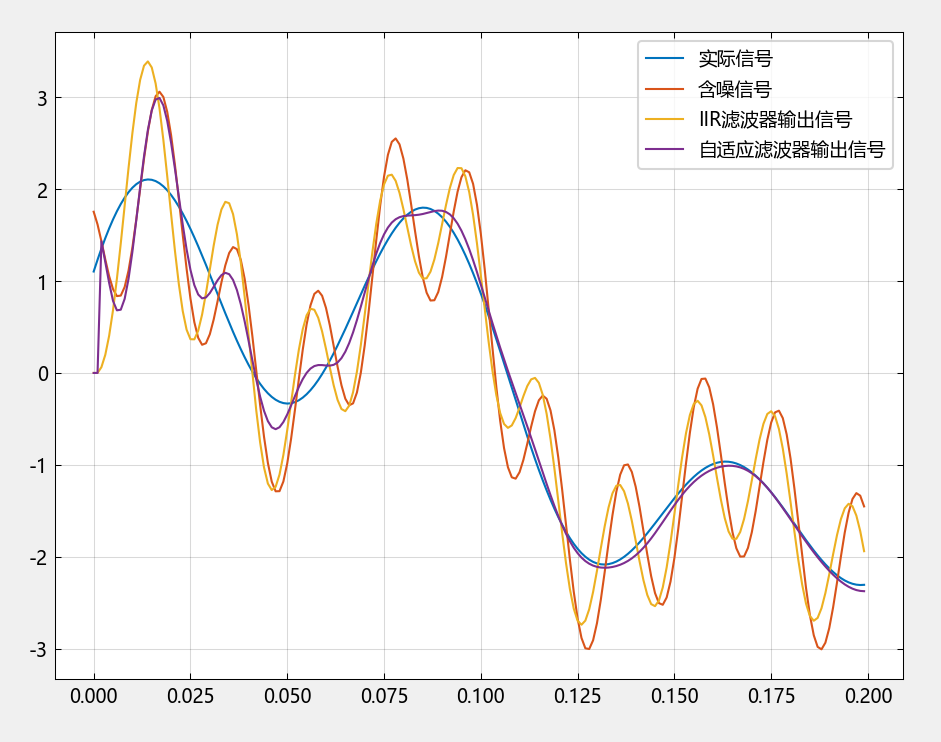
\includegraphics[width=0.8\linewidth]{图片/确定幅值滤波效果对比}
						\caption{确定幅值工频滤波效果对比}
						\label{确定幅值工频滤波效果对比}
					\end{subfigure}
					\begin{subfigure}{0.45\linewidth}
						\centering
						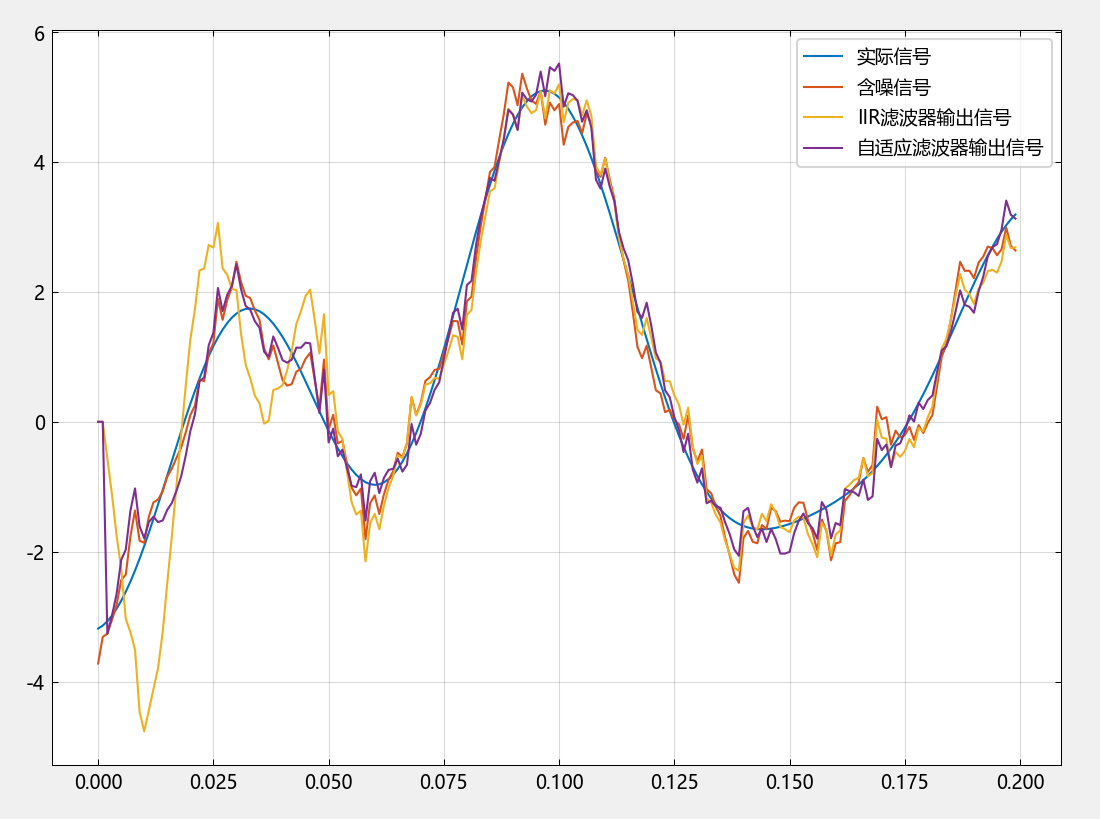
\includegraphics[width=0.85\linewidth]{图片/随机幅值滤波效果对比}
						\caption{随机幅值工频滤波效果对比}
						\label{随机幅值工频滤波效果对比}
					\end{subfigure}
					\caption{自适应滤波器和FIR工频滤波效果对比}
					\label{自适应滤波器和FIR工频滤波效果对比}
				\end{figure}
				从图\ref{确定幅值工频滤波效果对比}可看出，当工频幅值为定常数时，采用自适应滤波器滤除工频干扰，较传统的工频50Hz陷波器，能提供易于控制的宽带，无穷深的零点，以及自适应的跟踪干扰的精确频率和相位能力，防止有用数据丢失。自适应滤波算法不仅阶数低，具有自动调节参数的能力。\par
				从图\ref{随机幅值工频滤波效果对比}可看出，虽然工频噪声不断变化，发生多处毛刺，但是自适应滤波器能对原信号有更好的跟踪性能，自动适应噪声带来的突发影响。\par
				为了更直观的体现滤波器的性能，本文增大信号点数，统计了1000次滤波后均方值的直方图，以评价滤波器的工作效果，如下图所示：
				\begin{figure}[H]
					\centering
					\begin{subfigure}{0.45\linewidth}
						\centering
						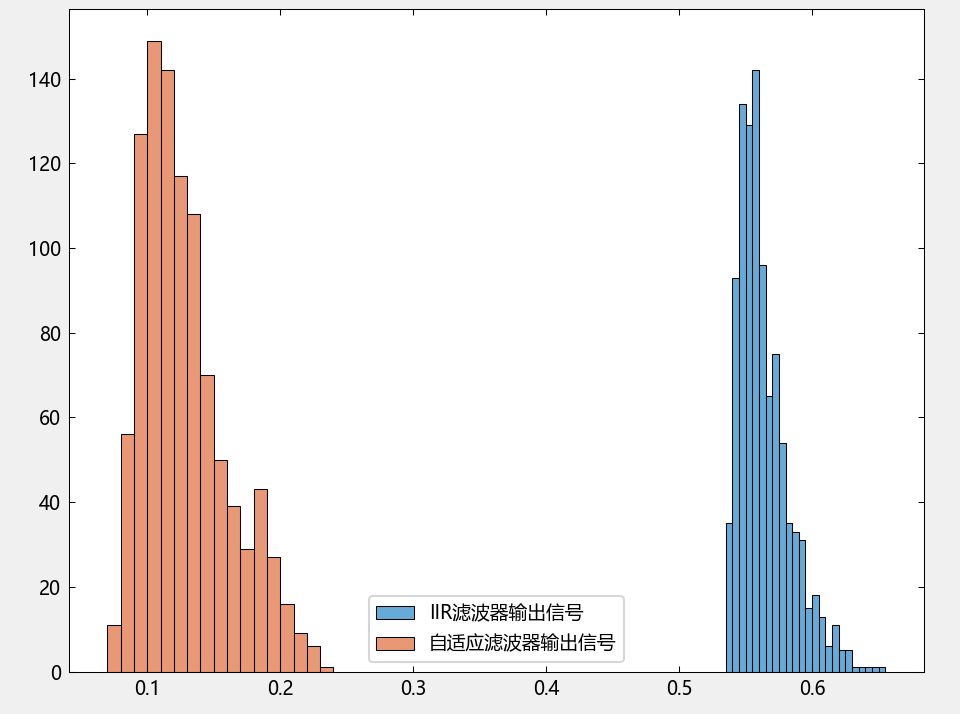
\includegraphics[width=0.8\linewidth]{图片/确定幅值滤波效果直方图对比}
						\caption{确定幅值工频滤波效果均方值统计}
						\label{确定幅值工频滤波效果均方值统计}
					\end{subfigure}
					\begin{subfigure}{0.45\linewidth}
						\centering
						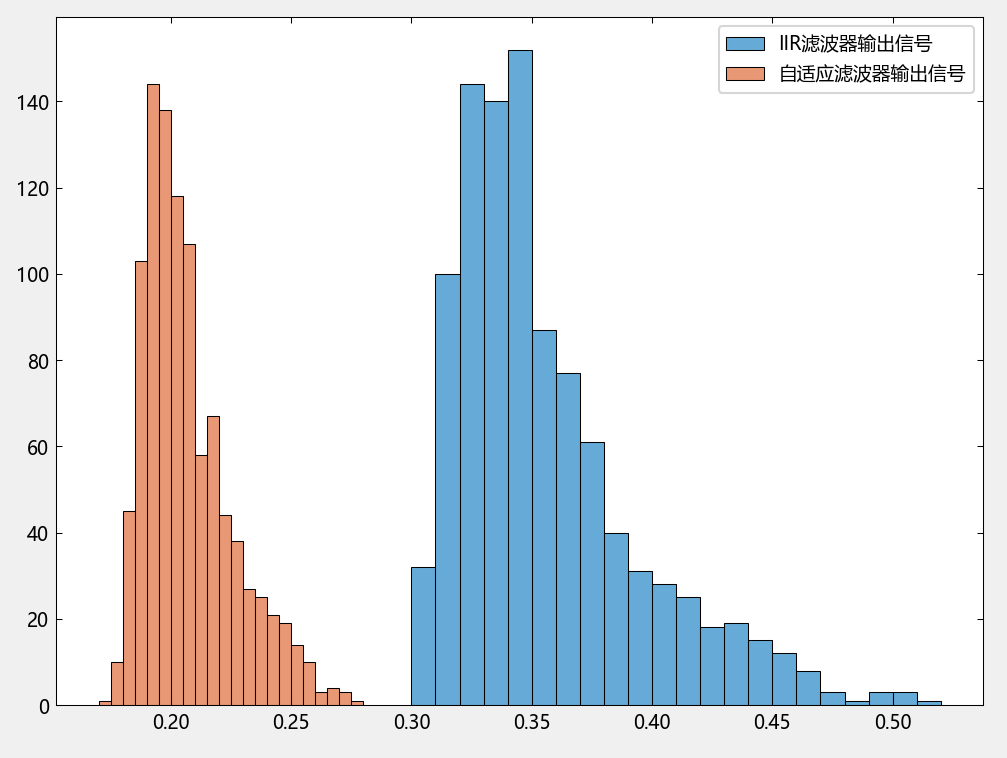
\includegraphics[width=0.82\linewidth]{图片/随机幅值滤波效果直方图对比}
						\caption{随机幅值工频滤波效果均方值统计}
						\label{随机幅值工频滤波效果均方值统计}
					\end{subfigure}
					\caption{自适应滤波器和FIR工频滤波效果均方值统计对比}
					\label{自适应滤波器和FIR工频滤波效果均方值统计对比}
				\end{figure}
		\subsection{基线偏移伪迹去除算法仿真}
			\subsubsection{算法实现}
				Mwork软件在TySignalProcessing函数库中给出了sgolayfilt函数以实现Savitzky-Golay滤波。\par
				其语法为：
				\begin{lstlisting}[language={Python}]
y = sgolayfilt(x, order, framelen)
				\end{lstlisting}
				其中order为滤波器阶数，framelen为帧长。\par
				将输入信号与滤波器输出信号相减后的信号即为去噪信号。
			\subsubsection{效果对比}
				Savitzky-Golay滤波器的性能很大程度上取决于窗口大小和多项式阶数的选择。这两个参数需要根据具体应用场景进行优化。\par
				窗口大小的选择需要考虑以下因素：\par
				小窗口适用于快速变化信号的处理。优势是能够保持信号的局部特征和快速变化，但噪声抑制效果可能不够理想；大窗口：适用于缓慢变化信号的处理。具有更好的噪声抑制效果，但可能会模糊信号的局部特征。\par
				多项式阶数k的选择需要权衡以下因素：\par
				低阶多项式适用于平滑变化的信号、具有较好的抗噪声能力、计算效率较高；高阶多项式适用于具有复杂局部结构的信号、能够更好地保持信号特征、需要注意过拟合风险。
				\begin{figure}[h]
					\centering
					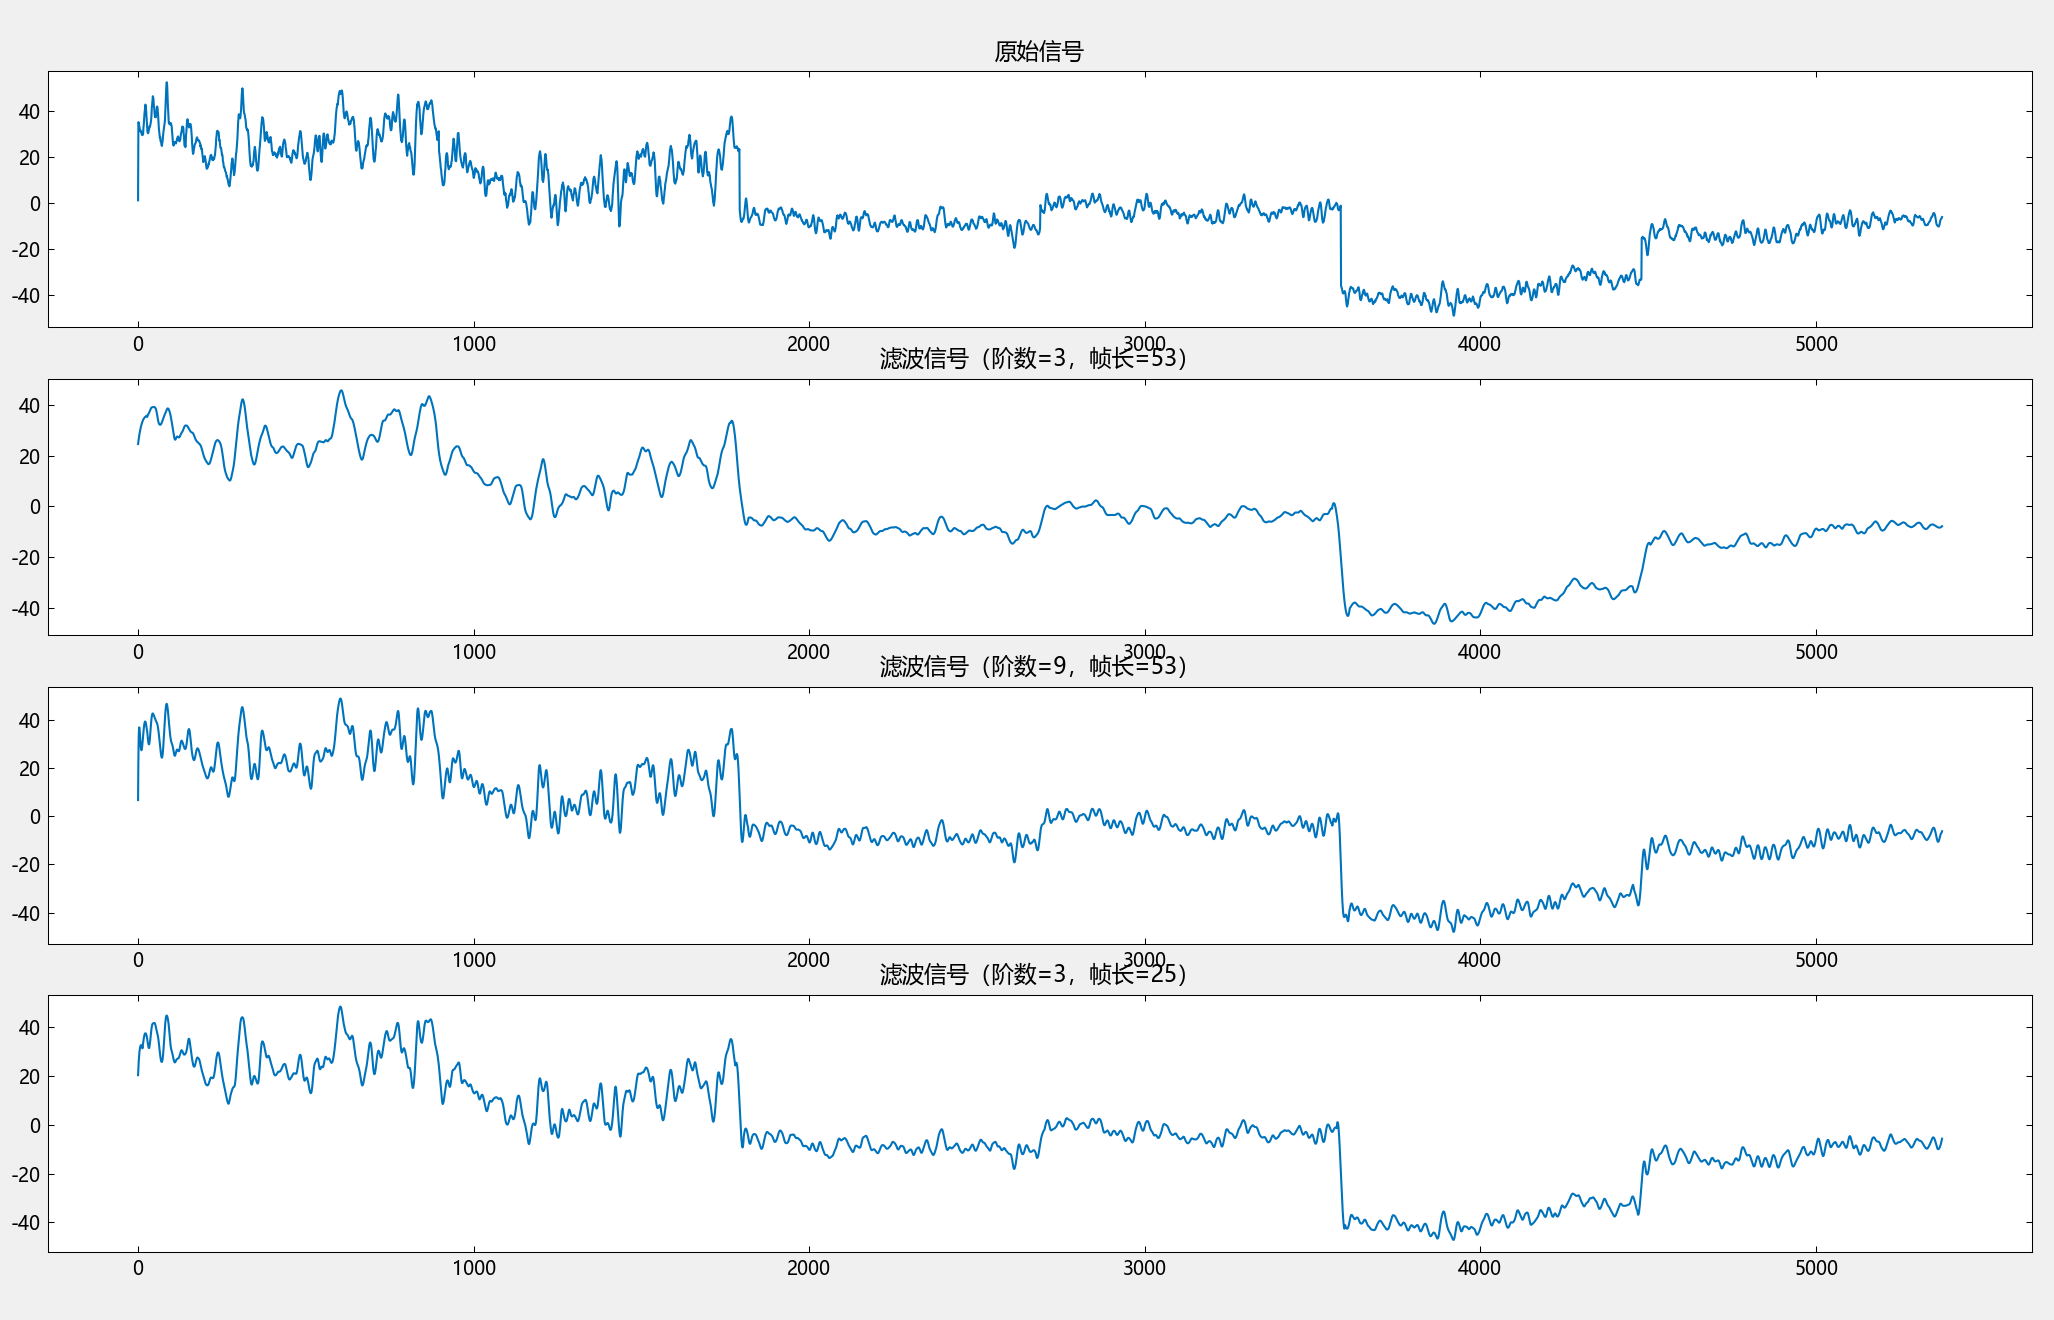
\includegraphics[width=0.8\linewidth]{图片/滤波器输出图像}
					\caption{不同阶次、不同窗口滤波器输出图像}
					\label{滤波器输出图像}
				\end{figure}
				图\ref{滤波器输出图像}针对公开脑电数据信号给出了不同阶次、不同窗口滤波器输出图像。\par
				对于高阶多项式滤波器，保留了信号的主要形态特征，清晰显示了信号的细微波动，对快速变化的信号成分响应更灵敏，并在信号起始和结束部分失真较小。但其运行结果可见残留的高频噪声，以及基线漂移抑制不足，整体信号仍呈现明显的向上漂移趋势。\par
				对于低阶多项式滤波器，其平滑效果显著，实现了优异的平滑效果，有效消除了整体信号的上升漂移趋势，并大幅降低了高频噪声成分，清晰呈现了信号的整体变化趋势。但会抑制峰值导致失真。\par
				综上所述选用3阶Savitzky-Golay滤波器来对原始信号进行平滑处理。这个平滑过程主要捕捉了信号中的低频成分，即基线漂移部分。因此，基线估计代表了信号中的慢变化趋势，即低频部分。\par
				进而可通过原始信号减去基线估计后得到基线校正后的信号。这样做的目的是去除信号中的低频漂移，使得校正后的信号在零基线附近波动。这有助于后续分析不受基线漂移的影响。
				\begin{figure}[h]
					\centering
					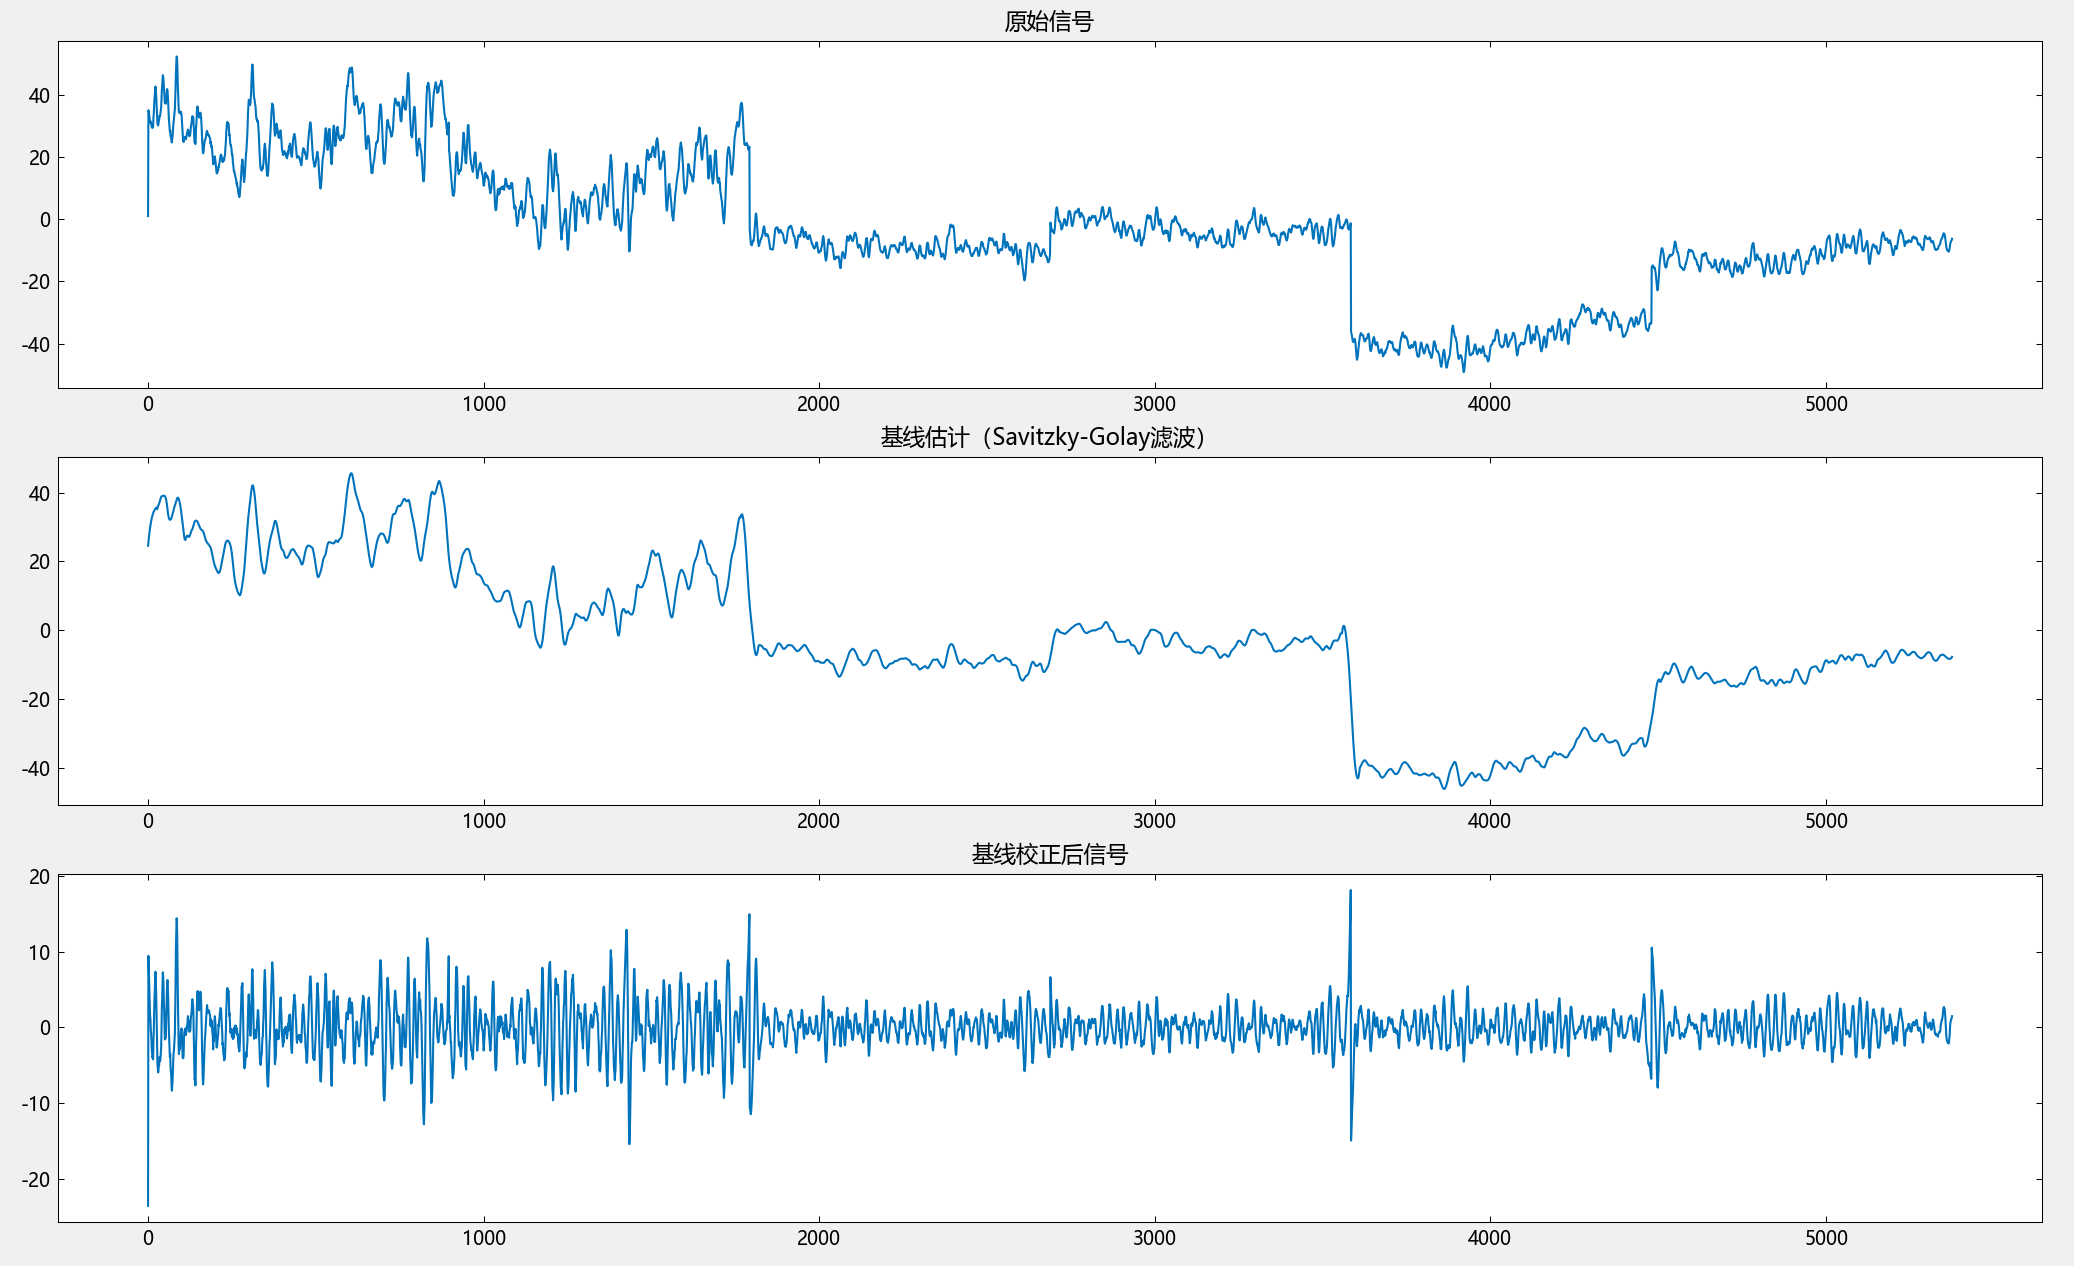
\includegraphics[width=0.8\linewidth]{图片/基线校正后信号}
					\caption{基线校正前后信号}
					\label{基线校正前后信号}
				\end{figure}
				如图\ref{基线校正前后信号}所示，基线估计是原始信号的低频成分，可能是由于仪器漂移、运动伪影等引起。基线校正后的信号是去除低频趋势后的信号，保留了原始信号中的中高频成分。并将基线校正后的信号作为后续频谱分析的初始信号。
			\subsection{脑电频段切片仿真}
				将上述基线校正的信号使用FSWT进行小波变换，给出信号时频域的强度图，如图\ref{频率切片小波变换时频图}所示。
				\begin{figure}[h]
					\centering
					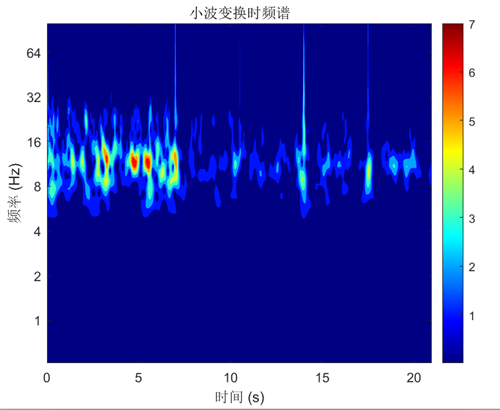
\includegraphics[width=0.6\linewidth]{图片/小波变换频谱}
					\caption{频率切片小波变换时频图}
					\label{频率切片小波变换时频图}
				\end{figure}
				该时频谱以时间为横轴、频率为纵轴，通过颜色强度反映信号能量分布。图中能量集中区域对应脑电活动的显著节律。低频段持续高能量，标志静息或睡眠状态；高频段的短暂爆发常与认知任务或外界刺激相关。\par
				对信号进行频率谱密度分析，其图像如下所示
				\begin{figure}[h]
					\centering
					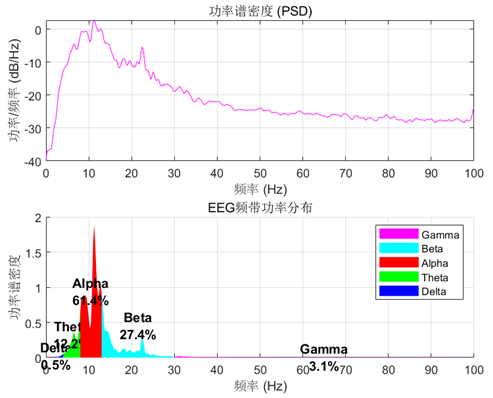
\includegraphics[width=0.6\linewidth]{图片/功率谱}
					\caption{频率切片小波变换功率谱}
					\label{频率切片小波变换功率谱}
				\end{figure}
				功率谱在0-100 Hz频率范围内呈现显著的非均匀性，能量主要集中在低频段。Alpha频段（8-13 Hz）以61.4\%的绝对优势成为主导节律，表明受试者处于深度放松或闭眼静息状态，符合后枕叶α波增强的典型生理特征。Theta（4-7 Hz）和Delta（<4 Hz）频段合并占比仅0.5\%，提示清醒状态下慢波活动受抑制；而Beta（13-30 Hz）占27.4\%，反映一定程度的认知活跃性或轻度焦虑状态。
	\section{结论与展望}
		\subsection{项目总结}
			脑电是典型的非平稳时变信号，具有复杂的时域、频域特征，同时又混杂着各类噪声信号。简单应用传统的时域、频域信号处理、统计方法已经不能简单的满足简单的要求了。因此几十年来，人们针对各类问题给出了多种多样的现代信号处理方案。\par
			本文基于前人的方案，整合整理提出了相对系统的滤波、去噪、统计的方案。利用自适应滤波器自动拟合去除50Hz工频信号；利用Savitzky-Golay滤波器滤除极低频信号及直流偏置；最后将滤波的信号通过频率切片小波变换，得到对应的时频图像。以分离出脑电的五类节律信号，针对节律信号开展具有科学意义的研究。\par
		\subsection{未来展望}
			本项目在脑电信号分析领域取得了显著的研究进展，成功构建了一个高效且精准的脑电信号特征分离体系。通过采用先进的滤波技术和算法，我们实现了对脑电信号的深度分析与处理，能够实时、量化地监测大脑的认知状态。这一体系不仅为教育注意力监测和心理障碍干预提供了可量化的神经反馈工具，而且推动了脑电分析技术从实验室向临床、教育场景的实用化发展，具有重要的科学价值和应用前景。
			在未来的工作中，计划将单路脑电信号扩展为十六导联信号，采集头部不同区域的脑电信号，分析不同区域信号间的关系，以进一步优化和完善脑电信号分析系统，以实现更全面、更精确的用户状态评估。
		
		
		
	\newpage
	\zihao{5}
	\bibliographystyle{gbt7714-numerical}
	\bibliography{tex}
	\newpage
	
	
	
\end{document}




